
\documentclass[tikz,border=5pt]{standalone}
\usepackage{tikz}
\usetikzlibrary{arrows.meta,calc,positioning}
\begin{document}
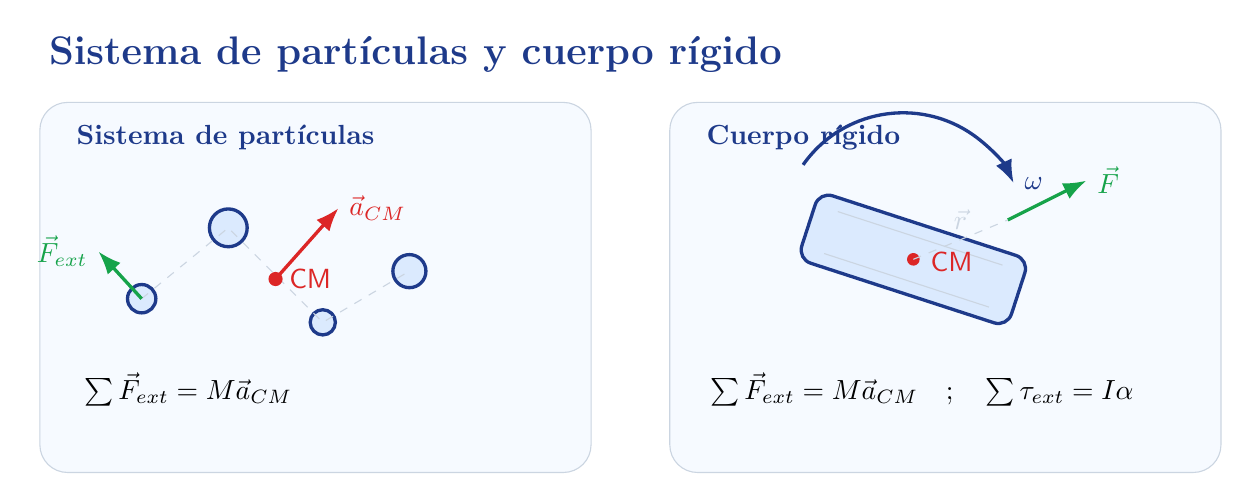
\begin{tikzpicture}[>=Latex, font=\sffamily]
\definecolor{brand}{HTML}{1E3A8A}
\definecolor{bluebox}{HTML}{DBEAFE}
\definecolor{green}{HTML}{16A34A}
\definecolor{red}{HTML}{DC2626}
\definecolor{grayline}{HTML}{CBD5E1}
\node[anchor=west, text=brand, font=\bfseries\Large] at (0,4.4) {Sistema de partículas y cuerpo rígido};
\node[draw=grayline, rounded corners=10pt, fill=bluebox!25, minimum width=7cm, minimum height=4.7cm, anchor=north west] (A) at (0,3.8) {};
\node[anchor=west, text=brand, font=\bfseries] at (.35,3.35) {Sistema de partículas};
\foreach \p/\r in {(1.3,1.3)/.18,(2.4,2.2)/.24,(3.6,1.0)/.16,(4.7,1.65)/.21}{\filldraw[fill=bluebox, draw=brand, line width=1.2pt] \p circle (\r);}
\draw[grayline,dashed] (1.3,1.3)--(2.4,2.2)--(3.6,1.0)--(4.7,1.65);
\fill[red] (3.0,1.55) circle (.09);
\node[red, right] at (3.05,1.55) {CM};
\draw[->, red, line width=1.2pt] (3.0,1.55)--(3.8,2.45) node[right] {$\vec a_{CM}$};
\draw[->, green, line width=1.2pt] (1.3,1.3)--(.75,1.9) node[left] {$\vec F_{ext}$};
\node[anchor=west] at (.45,.15) {$\sum \vec F_{ext}=M\vec a_{CM}$};
\node[draw=grayline, rounded corners=10pt, fill=bluebox!25, minimum width=7cm, minimum height=4.7cm, anchor=north west] (B) at (8.0,3.8) {};
\node[anchor=west, text=brand, font=\bfseries] at (8.35,3.35) {Cuerpo rígido};
\begin{scope}[shift={(11.1,1.8)}, rotate=-18]
\draw[fill=bluebox, draw=brand, line width=1.2pt, rounded corners=5pt] (-1.4,-.45) rectangle (1.4,.45);
\draw[grayline] (-1.1,-.28)--(1.1,-.28); \draw[grayline] (-1.1,.28)--(1.1,.28);
\fill[red] (0,0) circle (.08); \node[red, right] at (.1,0) {CM};
\end{scope}
\draw[->, brand, line width=1.2pt] (9.7,3.0) arc (145:25:1.55) node[right] {$\omega$};
\draw[->, green, line width=1.2pt] (12.3,2.3)--(13.3,2.8) node[right] {$\vec F$};
\draw[grayline,dashed] (11.1,1.8)--(12.3,2.3) node[midway,above] {$\vec r$};
\node[anchor=west] at (8.4,.15) {$\sum \vec F_{ext}=M\vec a_{CM}\quad ;\quad \sum \tau_{ext}=I\alpha$};
\end{tikzpicture}
\end{document}
